\subsection{Bestuur onderdeel}

Die bestuur onderdeel verskaf 'n generiese bestuursstelsel vir die
hantering van verskillende entiteite soos kampusse, allergieë, en
koshuise. Alle bestuursfunksies word gekonsolideer onder die SettingsScreen
en gebruik generiese bestuursdienste en -kontroleerders om konsekwente
funksionaliteit te verskaf.

\begin{figure}[H]
    \centering
    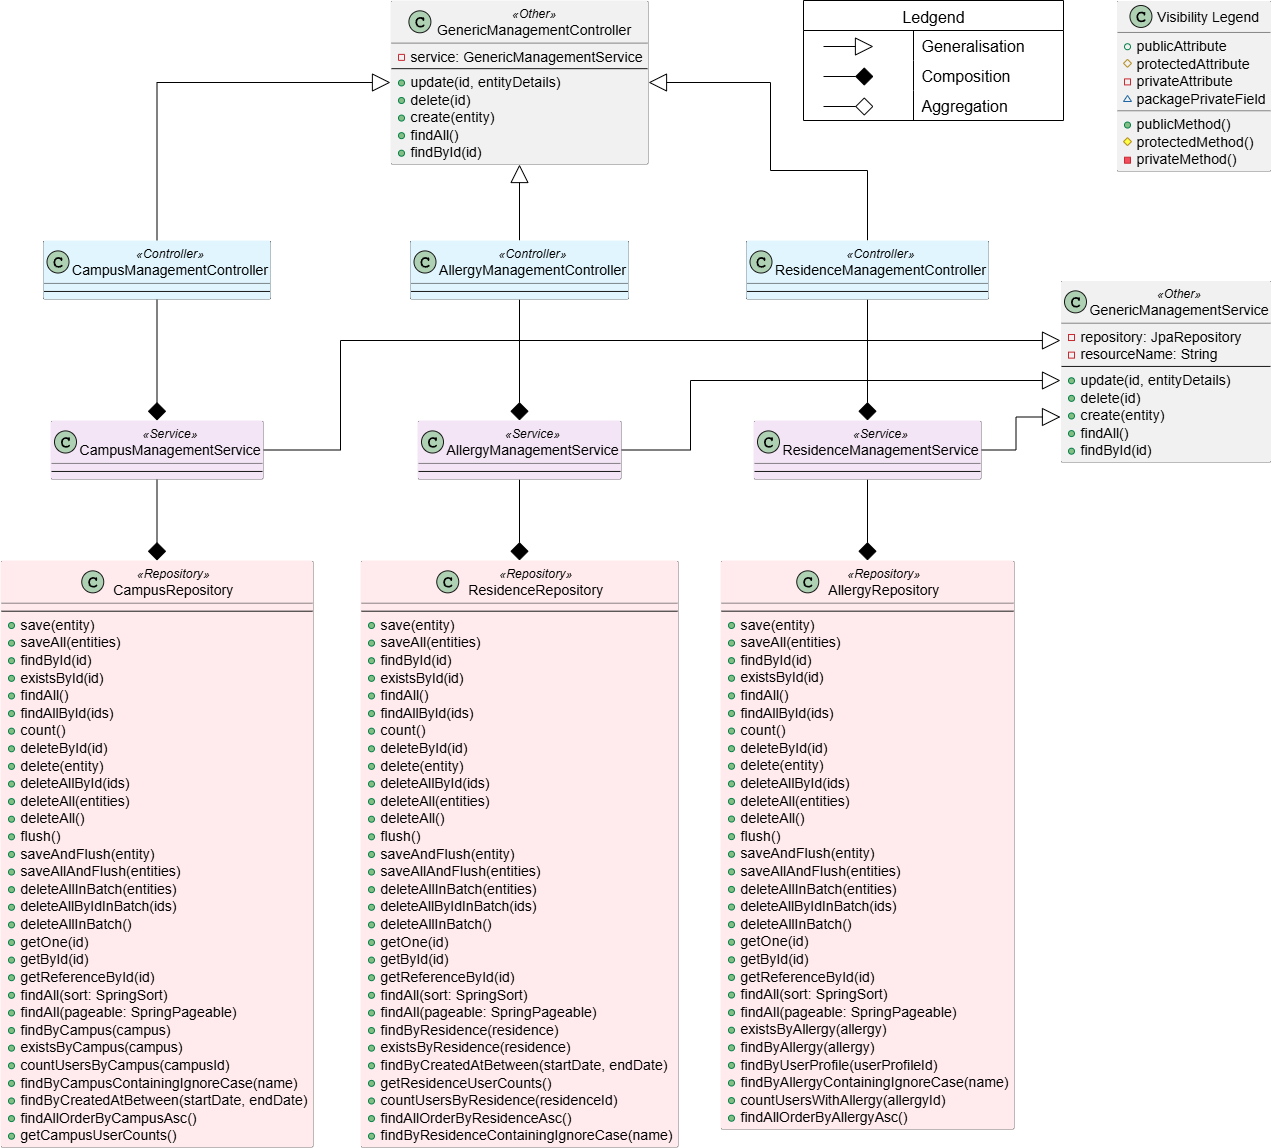
\includegraphics[width=\textwidth]{figures/class_diagrams/management-subsystem.png}
    \caption{Bestuur onderdeel klasdiagram}
    \label{fig:management_subsystem_class_diagram}
\end{figure}

Hier volg die CRC kaarte vir die belangrikste klasse in hierdie
onderdeel.

\textbf{SettingsScreen} bied sentrale toegang tot alle bestuursfunksies en navigeer na spesifieke bestuursseksies.

\vspace{1em}
\begin{table}[H]
\centering
\begin{tabular}{|p{0.4\textwidth}|p{0.4\textwidth}|}
    \hline
    \multicolumn{2}{|c|}{\textbf{SettingsScreen}} \\
    \hline
    \textbf{Verantwoordelikhede} & \textbf{Medewerkers} \\
    \hline
    Verskaf sentrale toegang tot alle bestuursfunksies \newline
    Navigeer na spesifieke bestuursseksies \newline
    Wys instellings en konfigurasie-opsies
    &
    GenericManagementController \\
    \hline
\end{tabular}
\caption{CRC vir SettingsScreen}
\label{tab:crc_settings_screen}
\end{table}

\textbf{GenericManagementController} hanteer CRUD-operasies vir alle bestuursentiteite en verskaf generiese REST-eindpunte.

\vspace{1em}
\begin{table}[H]
\centering
\begin{tabular}{|p{0.4\textwidth}|p{0.4\textwidth}|}
    \hline
    \multicolumn{2}{|c|}{\textbf{GenericManagementController}} \\
    \hline
    \textbf{Verantwoordelikhede} & \textbf{Medewerkers} \\
    \hline
    Hanteer CRUD operasies vir alle bestuursvolwasse entiteite \newline
    Verskaf generiese REST eindpunte \newline
    Roep spesifieke bestuursdienste aan
    &
    GenericManagementService \\
    \hline
\end{tabular}
\caption{CRC vir GenericManagementController}
\label{tab:crc_generic_management_controller}
\end{table}

\textbf{GenericManagementService} verskaf generiese CRUD-funksionaliteit, bestuur entiteitvalidasie en hanteer databasisinteraksies vir bestuursentiteite.

\vspace{1em}
\begin{table}[H]
\centering
\begin{tabular}{|p{0.4\textwidth}|p{0.4\textwidth}|}
    \hline
    \multicolumn{2}{|c|}{\textbf{GenericManagementService}} \\
    \hline
    \textbf{Verantwoordelikhede} & \textbf{Medewerkers} \\
    \hline
    Verskaf generiese CRUD funksionaliteit \newline
    Bestuur entiteit validasie \newline
    Hanteer database interaksies vir alle bestuursvolwasse entiteite
    &
    CampusManagementService \newline
    AllergyManagementService \newline
    ResidenceManagementService \\
    \hline
\end{tabular}
\caption{CRC vir GenericManagementService}
\label{tab:crc_generic_management_service}
\end{table}

\textit{Nota: Campus, Allergy, en Residence entiteite word bestuur as
spesialisasies van die generiese bestuursstelsel. Elke entiteit het sy eie
spesifieke bestuursdiens wat die GenericManagementService uitbrei vir
gespesialiseerde funksionaliteit.}
